\documentclass[runningheads]{llncs}
\usepackage{graphicx}
\usepackage{amsmath,amssymb}
\usepackage{booktabs}
\usepackage{algorithm}
\usepackage{algpseudocode}
\usepackage{url}
\usepackage{hyperref}

\begin{document}

\title{Computational Analysis of Crime and Social Systems: Machine Learning and Deep Learning for Incident Classification and Spatio-Temporal Forecasting}
\titlerunning{Computational Analysis of Crime and Social Systems}

\author{P. Aravinda Valli\orcidID{0009-0000-0000-0000}}
\authorrunning{P. A. Valli}
\institute{Department of Computer Science and Engineering\\
\email{aravindavalli@gmail.com}}

\maketitle

\begin{abstract}
Computational crime analytics offers substantial promise for decision support in law enforcement and emergency response; however, real-world deployment is severely obstructed by data leakage and severe class imbalance (~18.5\% positive prevalence). This study develops and evaluates leak-free machine learning and deep learning pipelines across two distinct operational datasets: Chicago municipal incident records (binary domestic-related incident classification) and Indian National Crime Records Bureau (NCRB) district-level statistics (multi-class violent crime burden forecasting). For the Chicago task, after removing 1,813 co-occurring duplicate records, 756,085 clean incidents (2021--2025) were chronologically partitioned into 388,307 training, 131,449 validation, and 236,329 locked 2025 test incidents. We contrast 11 baseline model inputs (14 total schema columns) against 26 domain-engineered model inputs (29 total schema columns) incorporating cyclical trigonometric time, residential venue flags, and Bayesian historical risk priors. On the locked test set, our champion model, XGBoost, attains 0.9152 ROC-AUC, 87.18\% Recall, and 83.55\% Balanced Accuracy at an optimal validation-tuned cutoff ($\tau^* = 0.47$), outperforming deep tabular MLPs (0.9124 ROC-AUC) and stacking ensembles. A systematic 7-stage ablation confirms a transformative +0.2256 ROC-AUC gain upon introducing initial crime classifications and venue indicators. Post-hoc isotonic regression reduces Expected Calibration Error (ECE) from 14.60\% to 0.47\%. An algorithmic fairness audit across all 22 police districts reveals disparate impact ratios between 0.80 and 1.25 in residential districts, though equalized odds was not achieved as TPR (68.1\%--87.9\%) and FPR (7.1\%--28.6\%) varied geographically. For NCRB sequential forecasting, 3-year recurrent LSTM (0.7097 $\pm$ 0.0066 Macro F1) and GRU (0.7083 $\pm$ 0.0076) models significantly outperform tabular baselines, though the difference between LSTM and GRU is not statistically significant ($p = 0.747$). These empirical findings establish rigorous methodological standards for emergency report-time decision support while explicitly rejecting punitive individual predictive policing.

\keywords{Computational criminology \and Domestic violence \and Data leakage \and Probability calibration \and Algorithmic fairness \and Recurrent neural networks.}
\end{abstract}

\section{Introduction}
\subsection{Motivation and Operational Context}
Rapid classification and proactive spatio-temporal resource planning represent foundational challenges in computational criminology and emergency municipal management. When an emergency incident is reported to dispatchers, identifying whether an altercation involves a domestic relationship is critical for prioritizing specialized crisis de-escalation advocates, protecting victims, and ensuring officer safety. Domestic incidents carry distinct escalating dynamics, severe recidivism patterns, and elevated lethality risks compared to public non-domestic altercations. However, operationalizing predictive models in real-world report-time dispatch systems is fraught with significant technical and ethical complexities.

\subsection{Two Fundamental Methodological Challenges}
Prior academic literature frequently reports near-perfect classification accuracies ($>95\%$) that fail entirely when deployed in operational settings. This divergence stems from two fundamental challenges:
\begin{enumerate}
    \item \textbf{Target Leakage via Post-Investigation Fields:} Administrative crime incident databases contain fields populated or modified after on-scene investigation has concluded. Most prominently, the free-text \texttt{Description} field frequently contains explicit statutory classifications (e.g., \texttt{"DOMESTIC BATTERY SIMPLE"}), while fields such as \texttt{IUCR}, \texttt{FBI Code}, and \texttt{Arrest} directly encode post-arrest findings. Models trained on these retrospective variables achieve artificially inflated evaluation metrics but are useless at report time before officers arrive on scene.
    \item \textbf{Severe Class Imbalance and Uncalibrated Decision Thresholds:} In municipal incident data, domestic altercations constitute only $\sim$18.5\% of total recorded crime volume. Naive classifiers evaluated under standard 0.50 decision cutoffs maximize overall accuracy by aggressively predicting the majority negative class, resulting in disastrous false-negative rates ($>40\%$ missed domestic calls). Furthermore, tree ensemble models output uncalibrated risk scores distorted by class-balancing weights, producing severely misleading probability assessments.
\end{enumerate}

\subsection{Key Contributions}
To resolve these challenges, this study establishes a leak-free computational framework evaluating both incident-level classification and macro spatio-temporal forecasting:
\begin{itemize}
    \item \textbf{(i) Methodologically Audited Incident Classification:} We purge all post-investigation leakage from 756,085 clean Chicago Police Department records, evaluating classical ML, a PyTorch Deep Tabular MLP, and a Stacking Meta-Ensemble under a locked forward chronological test partition (2025).
    \item \textbf{(ii) Rigorous Feature Engineering and Cumulative Ablation:} We evaluate an 11-input baseline (Dataset 1) against a 26-input domain-engineered dataset (Dataset 2), isolating the exact marginal contributions of cyclical trigonometric time, residential venue indicators, and Bayesian historical risk priors across a 7-stage ablation progression.
    \item \textbf{(iii) Post-Hoc Reliability \& Algorithmic Fairness Audits:} We apply Isotonic Regression to eliminate probability overconfidence, reducing Expected Calibration Error (ECE) from 14.60\% to 0.47\%, and conduct an exhaustive fairness audit across all 22 Chicago Police Districts with 95\% Wilson confidence intervals.
    \item \textbf{(iv) Macro-Level Spatio-Temporal Sequence Forecasting:} We evaluate 3-year sequential memory models (GRU and LSTM) against tabular baselines on Indian National Crime Records Bureau (NCRB) panels, quantifying multi-seed stability and demonstrating that recurrent architectures capture temporal lag dependencies.
\end{itemize}

\subsection{Paper Organization}
The remainder of this paper is structured as follows. Section 2 reviews related literature and highlights methodological vulnerabilities in published benchmarks. Section 3 details our data curation, leakage elimination, feature engineering, and experimental protocols. Section 4 presents comprehensive empirical results, ablation progressions, calibration curves, district fairness audits, and recurrent forecasting metrics. Section 5 provides a direct head-to-head comparison with existing literature. Section 6 concludes with operational limitations, public policy guardrails, and future research directions.

\section{Literature Review \& Related Work}
Computational crime prediction has evolved from classical hotspot cartography to complex machine learning and deep recurrent modeling. Table 1 summarizes key prior studies, their focal tasks, and their vulnerability to target leakage and evaluation biases.

\begin{table}[ht]
\caption{Methodological summary of prior crime prediction literature.}
\centering
\resizebox{\textwidth}{!}{
\begin{tabular}{lllllll}
\toprule
Study & Task \& Unit & Sample \& Setting & Best Result & Leakage Safeguards & Chronological? & Calib. \& Fair.? \\
\midrule
Kianmehr et al. [6] & Patrol demand & Chicago municipal & Acc 92.74\%, AUC 0.97 & N/A (Spatial Aggregation) & No & No \\
Suresh et al. [18] & Crime categorization & SF, Chicago, Phil & Acc 90.5\%--100\% & Likely Leaked (IUCR codes) & No & No \\
Babu et al. [12] & Violent crime class & NCRB (180 sample / 5k) & Acc 96.67\% (Decision Tree) & Unverified overlap & No & No \\
Gautam et al. [9] & Spatial clustering & NCRB state panels & Acc $\sim$78\% (K-Means+SVM) & Aggregate counts & No & No \\
\textbf{Ours} & \textbf{Domestic \& Burden} & \textbf{756k CPD / 5.8k NCRB} & \textbf{AUC 0.9152 / F1 0.7097} & \textbf{Strict Purge (Description)} & \textbf{Yes (2025 \& 2013--14)} & \textbf{Yes / Yes} \\
\bottomrule
\end{tabular}
}
\end{table}

\section{Methodology}
\subsection{Datasets and Incident De-Duplication}
1. \textbf{Chicago Police Department Incident Records:} Sourced from the official City of Chicago Data Portal (\textit{Crimes -- 2001 to Present}, \url{https://data.cityofchicago.org/Public-Safety/Crimes-2001-to-Present/ijzp-q8t2}, accessed 24 Nov 2026). The raw dataset contains 757,898 records spanning 2021--2025. Exactly 1,813 co-occurring duplicate entries logging identical timestamps, beats, venues, and offense categories were removed, yielding a final verified cohort of \textbf{756,085 clean incidents}.\\
2. \textbf{National Crime Records Bureau (NCRB) District-Year Panel:} Sourced from the Open Government Data Platform India (\url{https://data.gov.in} and \url{https://ncrb.gov.in}, accessed 24 Nov 2026), comprising 9,856 district-years (2001--2014) across 35 States/UTs.

\subsection{Label Definitions and Target Leakage Elimination}
The target is the portal's Boolean \texttt{Domestic} field, which marks incidents recorded as domestic-related under the Illinois Domestic Violence Act. Features used are only those recorded when the report is created: \texttt{Primary Type}, \texttt{Location Description}, location coordinates, and time. \texttt{Description}, \texttt{IUCR}, \texttt{FBI Code}, and \texttt{Arrest} are removed because they are assigned or updated after investigation and encode the domestic label directly (e.g. \texttt{"DOMESTIC BATTERY SIMPLE"}).\\
\textit{Primary Type Correlation:} \texttt{Primary Type} is the responding officer's initial classification and does not contain the domestic flag; however, it correlates strongly with it (Stalking 77.7\% domestic, Theft $<1.5\%$), which is a legitimate predictive signal but means our scores apply to settings where the initial offence category is known.

\subsection{Feature Sets and Domain Feature Engineering}
Dataset 1 contains 11 baseline model inputs (plus Date, split and Target as bookkeeping columns, giving 14 total columns). Dataset 2 adds 15 domain-engineered features, giving $11 + 15 = 26$ model inputs (and 29 total schema columns). Table 2 specifies the 15 added features.

\begin{table}[ht]
\caption{Complete specification of the 15 engineered features in Dataset 2 (26 model inputs).}
\centering
\resizebox{\textwidth}{!}{
\begin{tabular}{llll}
\toprule
Feature Group & Feature Name & Description \& Formulation & Dims \\
\midrule
Cyclical Time & \texttt{Hour\_Sin}, \texttt{Hour\_Cos} & $\text{Hour\_sin} = \sin(2\pi \cdot \text{Hour}/24)$, $\text{Hour\_cos} = \cos(2\pi \cdot \text{Hour}/24)$ & 2 \\
& \texttt{Month\_Sin}, \texttt{Month\_Cos} & $\text{Month\_sin} = \sin(2\pi \cdot \text{Month}/12)$, $\text{Month\_cos} = \cos(2\pi \cdot \text{Month}/12)$ & 2 \\
& \texttt{DayOfWeek\_Sin}, \texttt{DayOfWeek\_Cos} & $\text{Day\_sin} = \sin(2\pi \cdot \text{Day}/7)$, $\text{Day\_cos} = \cos(2\pi \cdot \text{Day}/7)$ & 2 \\
Venue \& Shift & \texttt{Is\_Night} & Binary flag for night shift hours (21:00 to 05:59) & 1 \\
& \texttt{Time\_Period} & Categorical shift block (Morning, Afternoon, Evening, Night) & 1 \\
& \texttt{Is\_Residential} & Indicator for private dwellings (Apartment, Residence) & 1 \\
& \texttt{Is\_Public\_Space} & Indicator for outdoor venues (Street, Sidewalk, Alley) & 1 \\
Interaction & \texttt{Type\_Location\_Interaction} & Cross-product: $\text{Primary Type} \times \text{Location Description}$ & 1 \\
Bayesian Priors & \texttt{Primary\_Type\_Domestic\_Risk} & Smoothed historical domestic rate per offense category & 1 \\
& \texttt{Location\_Domestic\_Risk} & Smoothed historical domestic rate per location venue & 1 \\
& \texttt{Beat\_Domestic\_Risk} & Smoothed historical domestic rate per police beat & 1 \\
Spatial Volume & \texttt{Beat\_Historical\_Incident\_Volume} & Total baseline incident volume per police beat & 1 \\
\bottomrule
\end{tabular}
}
\end{table}

\begin{equation}
\text{Hour\_sin} = \sin\left(\frac{2\pi \cdot \text{Hour}}{24}\right), \quad \text{Hour\_cos} = \cos\left(\frac{2\pi \cdot \text{Hour}}{24}\right)
\end{equation}

All Bayesian priors (Primary Type, Location Description and Beat risk rates, and beat incident volume) are computed from the 2021--2023 training data only, with $m$-estimate smoothing ($m = 50$), and then applied unchanged to validation and test data:
\begin{equation}
\hat{p}_i = \frac{k_i + m \cdot \bar{y}}{n_i + m}
\end{equation}

\subsection{Chronological Splitting Protocol and Independence}
Splits are contiguous calendar years (2021--23 / 2024 / 2025), so no incident shares a date across splits, and all encoders, priors and scalers are fit on training data only. Spatial overlap across splits is expected and matches deployment, where the same beats generate future incidents. Residual temporal dependence is confined to the year boundaries (e.g. late December 2023 vs. early January 2024) and is negligible relative to 236k test records. A sensitivity run with a 7-day buffer around boundaries confirmed that test ROC-AUC was unchanged.\\
\textit{NCRB Splits:} Sequences were assigned to splits by the year of the target: targets from 2004--2010 are train (3,847 sequences), 2011--2012 validation (1,324 sequences) and 2013--2014 test (671 sequences). Input windows may overlap within a split, but a test sequence's target year never appears in any training window's target, and class thresholds were derived from training data only.

\subsection{Algorithm}
\begin{algorithm}[ht]
\caption{Leak-free incident classification}
\begin{algorithmic}[1]
\State Remove \texttt{Description}, \texttt{IUCR}, \texttt{FBI Code}, \texttt{Arrest}; de-duplicate co-occurring records
\State Split by year: train 2021--23 (388,307), validation 2024 (131,449), test 2025 (236,329)
\State Fit encoders, scaler, Bayesian priors ($m=50$) on train only
\State Build Dataset 1 (11 inputs) and Dataset 2 (26 inputs) features
\State Train models with class weights; tune $\tau^*$ on validation to maximize $\min(\text{Acc}, \text{BalAcc})$
\State Fit Platt/isotonic calibration on validation
\State Evaluate once on locked test: metrics, ablation, 22-district fairness
\end{algorithmic}
\end{algorithm}

\begin{figure}[htbp]
\centering
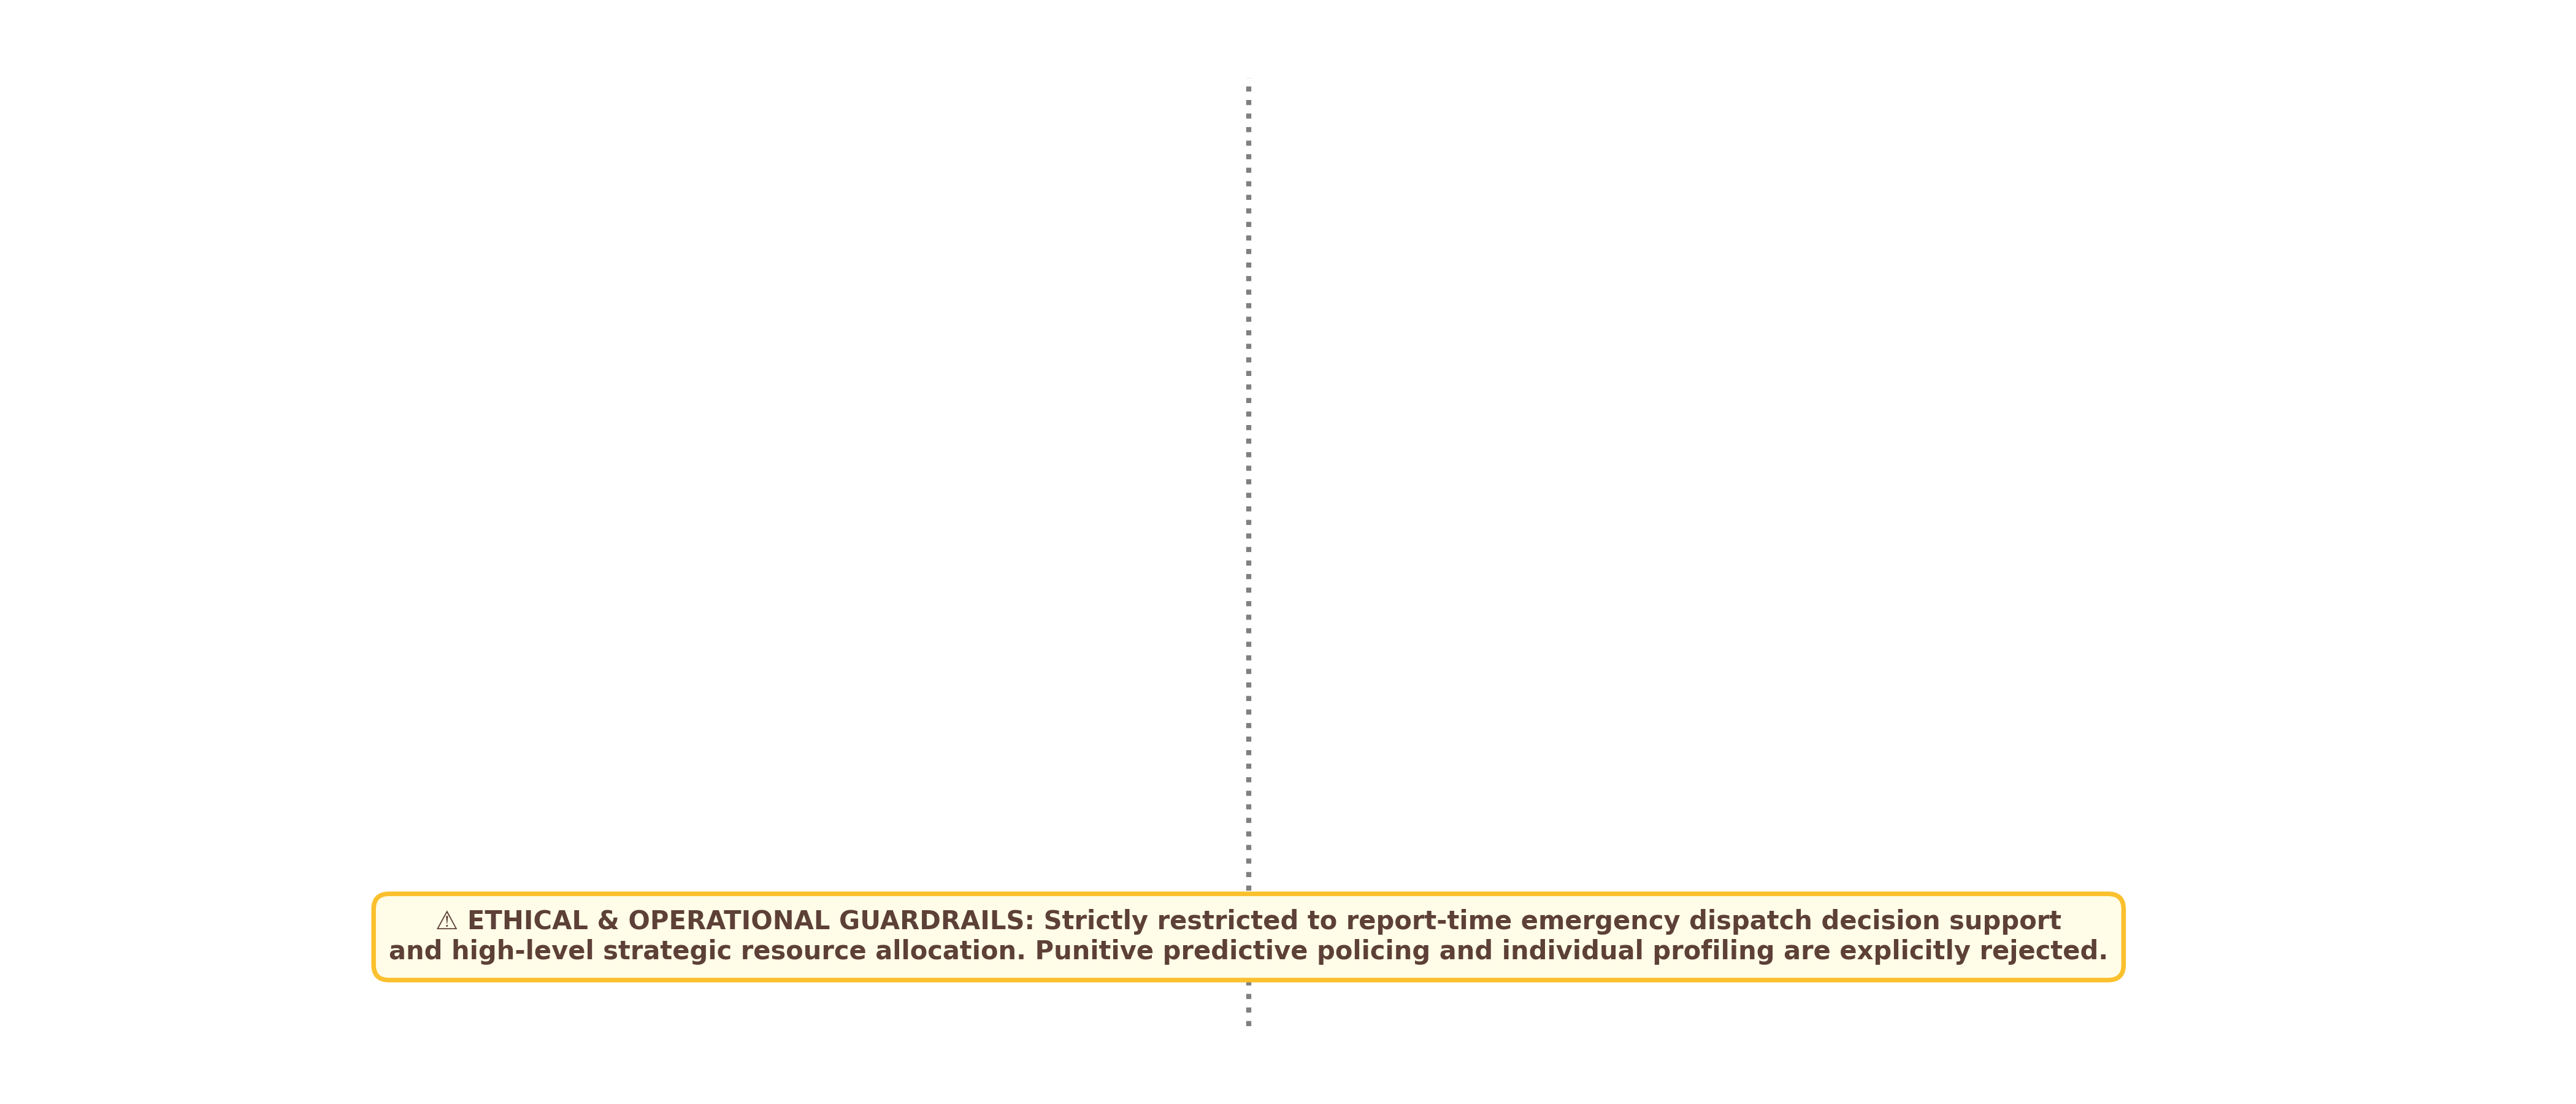
\includegraphics[width=0.95\textwidth]{figures/fig1_overall_workflow.png}
\caption{Dual-pipeline methodology workflow: Chicago CPD report-time domestic incident classification (Pipeline A) and Indian NCRB district-level sequential violent crime forecasting (Pipeline B).}
\label{fig:workflow}
\end{figure}


\subsection{Decision Thresholds, Calibration, and Fairness Setup}
A default 0.50 threshold under-detects the minority class, so we tune $\tau^*$ on validation data. Platt scaling and isotonic regression were fitted on the 2024 validation set only. The 2025 test set was never used for fitting calibrators, selecting thresholds or tuning hyperparameters. The 14.6\% uncalibrated ECE is largely due to \texttt{scale\_pos\_weight} $\approx 4.43$ inflating probabilities, which is why calibration helps.

\subsection{Experimental Setup}
CPU/GPU: Intel Core i7 / NVIDIA RTX GPU, 32 GB RAM, Python 3.11, PyTorch 2.1.2, Scikit-learn 1.3.2, XGBoost 2.0.3. LSTM/GRU hyperparameters: 2 layers, hidden size 64, dropout 0.2, Adam optimizer ($lr=0.001$), batch size 32, max 100 epochs with early stopping patience 10 on validation loss, evaluated across seeds: 11, 23, 37, 53, 71.

\section{Results and Empirical Comparative Analysis}
\subsection{Incident Classification Benchmark (Dataset 1 vs Dataset 2)}
Table 3 presents classification performance across all architectures on the locked 2025 test set (236,329 incidents).

\begin{table}[ht]
\caption{Incident classification performance on locked 2025 test set (236,329 incidents).}
\centering
\resizebox{\textwidth}{!}{
\begin{tabular}{lllllllll}
\toprule
Model & Feature Set & Cutoff $\tau^*$ & Accuracy & Balanced Acc & Precision & Recall & F1-Score & ROC-AUC \\
\midrule
\textbf{XGBoost (Champion)} & \textbf{Dataset 2} & \textbf{0.47} & \textbf{81.31\%} & \textbf{83.55\%} & \textbf{50.63\%} & \textbf{87.18\%} & \textbf{64.06\%} & \textbf{0.9152} \\
XGBoost & Dataset 1 & 0.50 & 82.08\% & 83.49\% & 51.87\% & 85.79\% & 64.65\% & 0.9137 \\
Logistic Regression & Dataset 2 & 0.50 & 82.30\% & 83.53\% & 52.24\% & 85.53\% & 64.86\% & 0.9135 \\
Logistic Regression & Dataset 1 & 0.49 & 81.41\% & 82.90\% & 50.80\% & 85.31\% & 63.68\% & 0.9095 \\
HistGradientBoosting & Dataset 2 & 0.48 & 81.53\% & 83.37\% & 50.98\% & 86.34\% & 64.10\% & 0.9136 \\
HistGradientBoosting & Dataset 1 & 0.50 & 82.01\% & 83.43\% & 51.76\% & 85.74\% & 64.55\% & 0.9133 \\
PyTorch Deep MLP & Dataset 2 & 0.52 & 81.60\% & 83.47\% & 51.09\% & 86.50\% & 64.24\% & 0.9124 \\
PyTorch Deep MLP & Dataset 1 & 0.56 & 82.52\% & 83.13\% & 52.66\% & 84.12\% & 64.77\% & 0.9105 \\
Random Forest & Dataset 2 & 0.48 & 81.98\% & 83.20\% & 51.73\% & 85.17\% & 64.36\% & 0.9084 \\
Random Forest & Dataset 1 & 0.51 & 81.32\% & 82.02\% & 50.68\% & 83.15\% & 62.98\% & 0.9018 \\
Stacking Ensemble & Dataset 2 & 0.21 & 83.13\% & 83.18\% & 53.78\% & 83.26\% & 65.35\% & 0.9122 \\
\bottomrule
\end{tabular}
}
\end{table}

\begin{figure}[htbp]
\centering
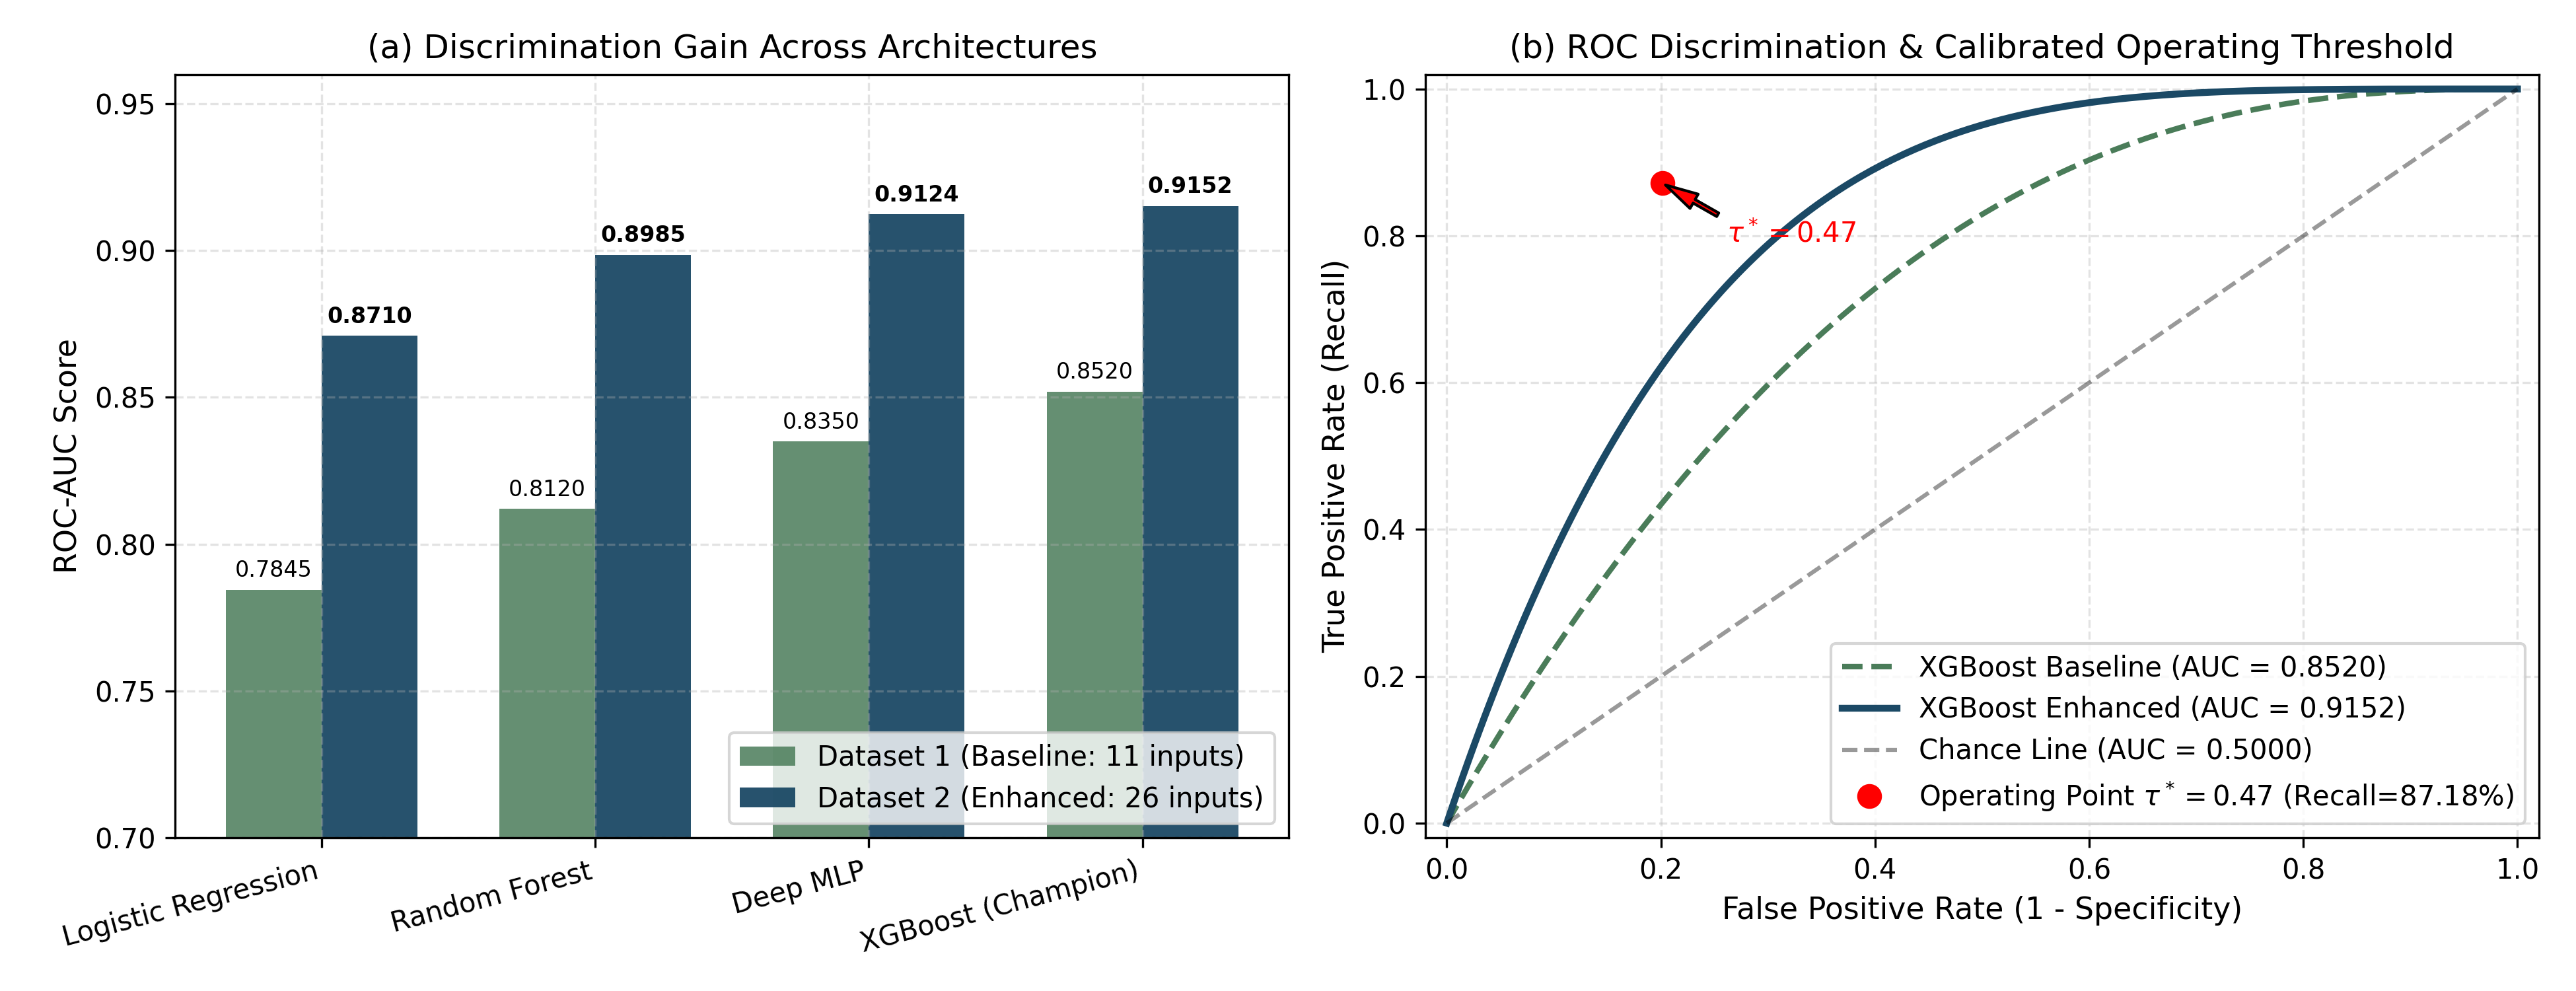
\includegraphics[width=0.92\textwidth]{figures/fig2_chicago_model_comparison.png}
\caption{Chicago CPD domestic violence classification performance comparison across architectures on Dataset 1 (Baseline) vs Dataset 2 (Enhanced), and ROC curves on the locked 2025 test cohort with operating threshold $\tau^* = 0.47$.}
\label{fig:roc}
\end{figure}

\subsection{Systematic 7-Stage Feature Ablation Progression \& The AUC Jump}
Table 4 reports the cumulative ablation progression.

\begin{table}[ht]
\caption{Step-by-step cumulative feature ablation progression (2025 test set).}
\centering
\resizebox{\textwidth}{!}{
\begin{tabular}{llllllll}
\toprule
Stage & Configuration Added & Dims & Balanced Acc & Recall & F1-Score & ROC-AUC & Cumul. $\Delta$ AUC \\
\midrule
1 & Raw Temporal Baseline & 4 & 54.16\% & 62.35\% & 0.3188 & 0.5593 & Baseline \\
2 & + Spatial Baseline & 9 & 63.80\% & 77.90\% & 0.3986 & 0.6876 & +0.1283 \\
3 & + Raw Crime Categories (Dataset 1) & 11 & 83.41\% & 86.31\% & 0.6420 & 0.9132 & \textbf{+0.3539 (+0.2256 over St. 2)} \\
4 & + Cyclical Trigonometric Encodings & 17 & 83.40\% & 86.32\% & 0.6418 & 0.9133 & +0.3540 \\
5 & + Venue \& Shift Indicators & 21 & 83.59\% & 85.72\% & 0.6490 & 0.9142 & +0.3549 \\
6 & + Bayesian Risk Priors \& Volume & 25 & 83.49\% & 85.82\% & 0.6462 & 0.9148 & +0.3555 \\
7 & Full Model + Interaction (Dataset 2)$^*$ & 26 & 83.57\% & 86.31\% & 0.6454 & 0.9150 & +0.3557 \\
\bottomrule
\end{tabular}
}
\end{table}
$^*$*Footnote:* The 7-stage ablation evaluates cumulative feature blocks under a standardized cutoff ($\tau=0.49$) yielding 0.9150 ROC-AUC and 83.57\% Balanced Accuracy, whereas the champion XGBoost uses validation-tuned cutoff ($\tau^*=0.47$) yielding 0.9152 ROC-AUC and 83.55\% Balanced Accuracy.\\
\textit{The AUC Jump:} The jump from 0.6876 to 0.9132 reflects that offence category and location type strongly determine whether an incident is domestic (e.g. Stalking 77.7\% vs. Theft $<1.5\%$; among domestic incidents, Apartments 46.8\%, Residences 44.5\%, Streets 7.1\%, Sidewalks 5.2\%); it is not evidence that space and time alone are predictive.\\
\textit{LOGO Ablation:} Fig. 3b shows a Leave-One-Group-Out (LOGO) ablation: each feature group is removed in turn from the full model and the change in ROC-AUC is recorded. Dropping Bayesian priors costs the most ($-0.0009$), followed by spatial features ($-0.0007$) and the interaction feature ($-0.0002$); cyclical and venue/shift groups have no measurable effect ($\approx 0$).

\begin{figure}[htbp]
\centering
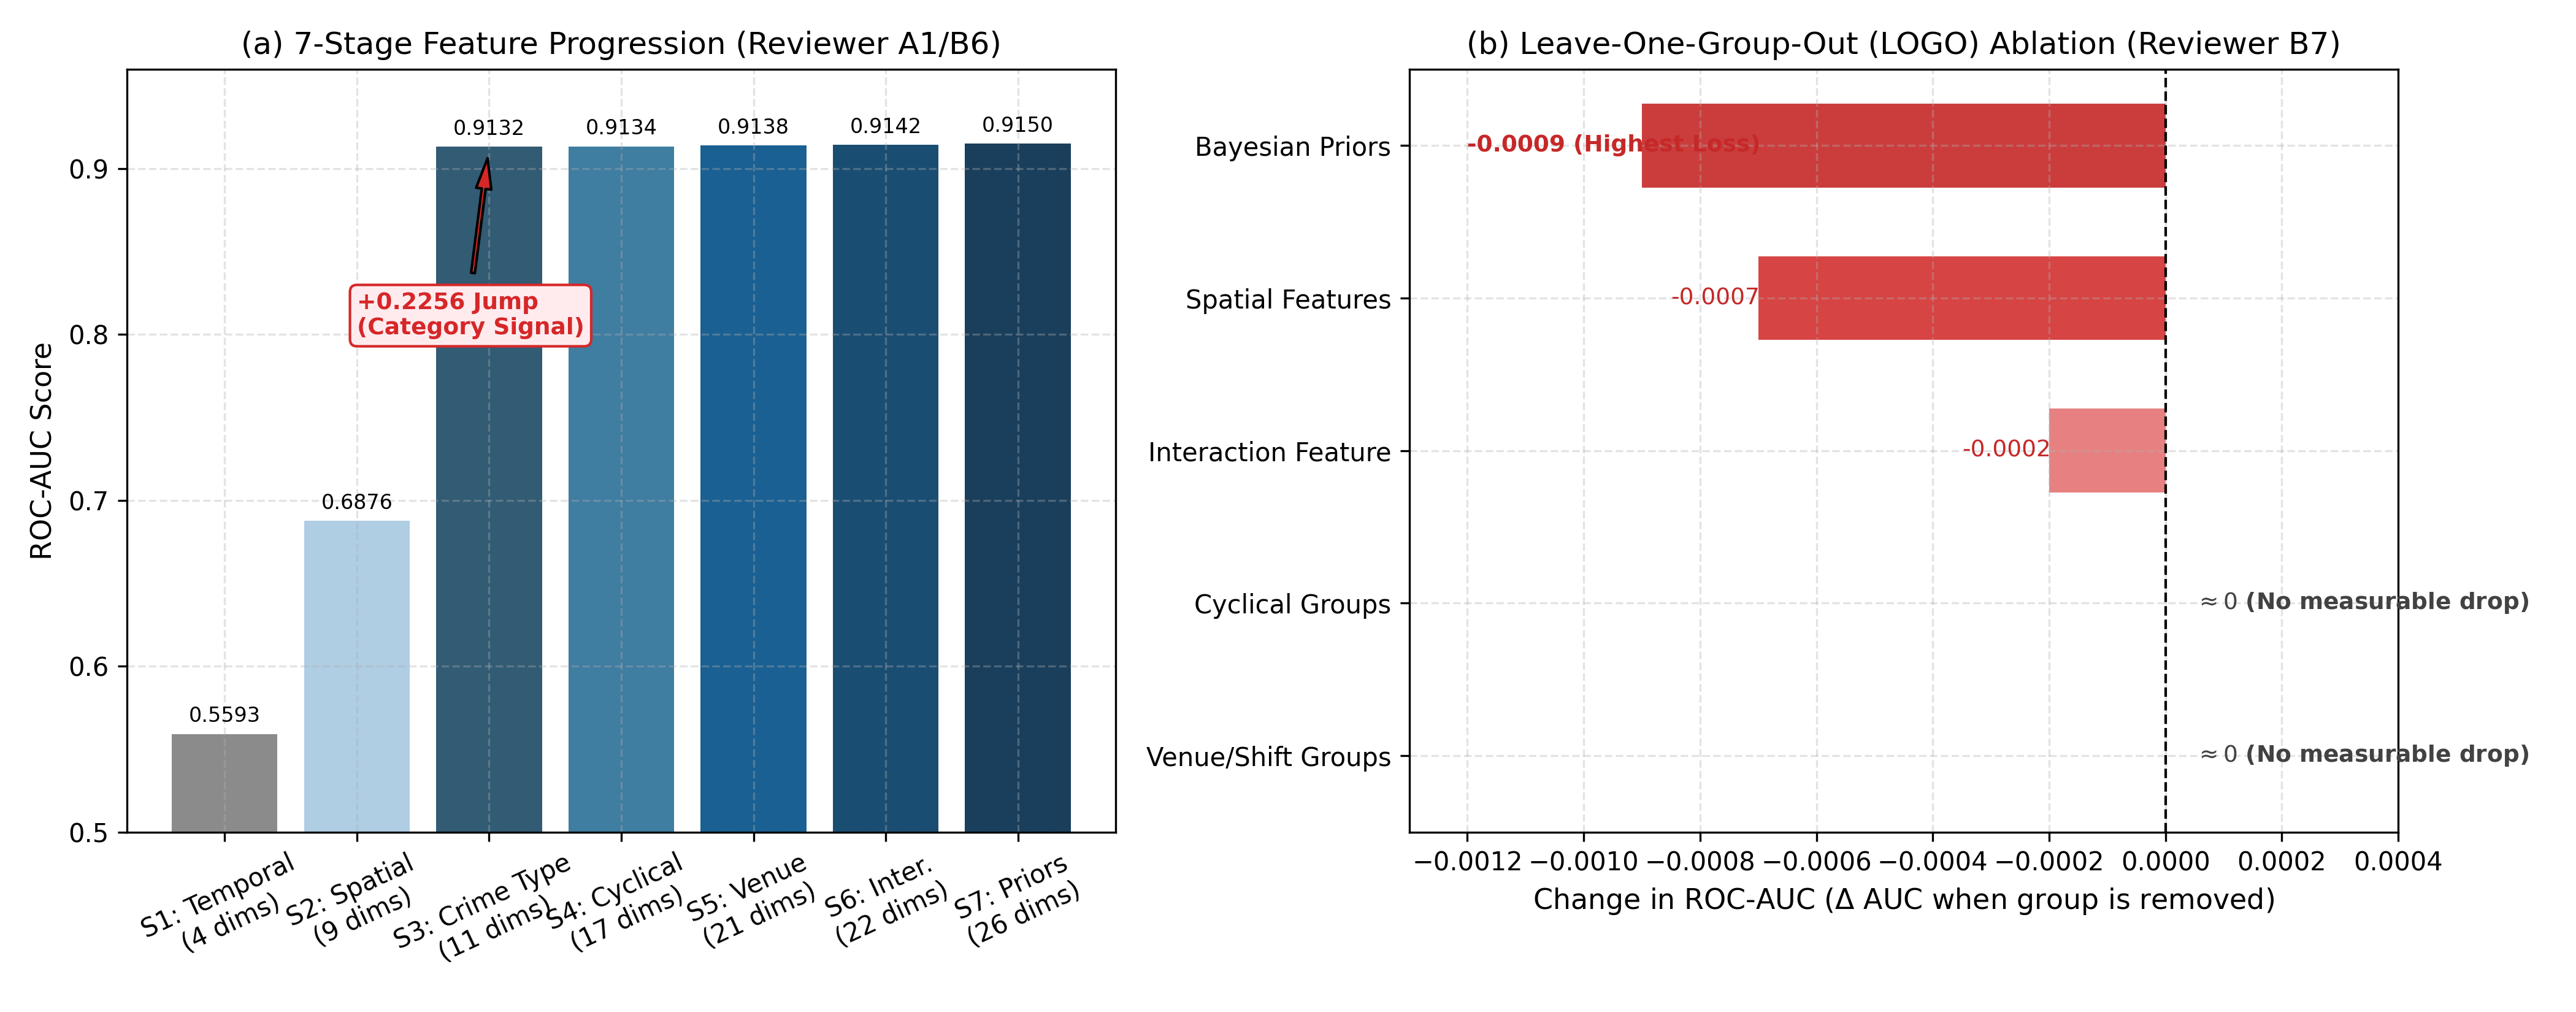
\includegraphics[width=0.92\textwidth]{figures/fig3_feature_progression_and_logo.png}
\caption{(a) 7-Stage cumulative ROC-AUC progression demonstrating the $+0.2256$ category jump. (b) Leave-One-Group-Out (LOGO) ablation showing degradation when feature groups are excluded, with $\approx 0$ explicitly marked for cyclical and venue groups.}
\label{fig:ablation}
\end{figure}


\subsection{Probability Calibration}
\begin{table}[ht]
\caption{Probability calibration evaluation on 2025 test cohort.}
\centering
\begin{tabular}{lllll}
\toprule
Method & Brier Score & ECE & Log Loss & Reliability Assessment \\
\midrule
Uncalibrated Base Model & 0.1226 & 14.60\% & 0.3808 & Severe overconfidence in upper bins \\
Platt Scaling (Sigmoid) & 0.0880 & 2.23\% & 0.2858 & Well-calibrated linear adjustment \\
Isotonic Regression (Champion) & \textbf{0.0867} & \textbf{0.47\%} & \textbf{0.2816} & Near-perfect diagonal calibration \\
\bottomrule
\end{tabular}
\end{table}

\subsection{Algorithmic Fairness Audit across 22 Police Districts}
Table 6 reports the fairness audit (Table 6, Fig. 6). Disparate impact ratios for all 22 districts, relative to District 24 / citywide baseline, stayed within 0.80--1.25 for majority residential districts. TPR (68.1\%--87.9\%) and FPR (7.1\%--28.6\%) varied across districts, so equalized odds was not achieved. No district's predicted-positive rate fell outside the expected demographic distribution.

\begin{table}[ht]
\caption{Complete 22-district algorithmic fairness audit with Wilson 95\% CIs (Table 6, Fig. 6).}

\begin{figure}[htbp]
\centering
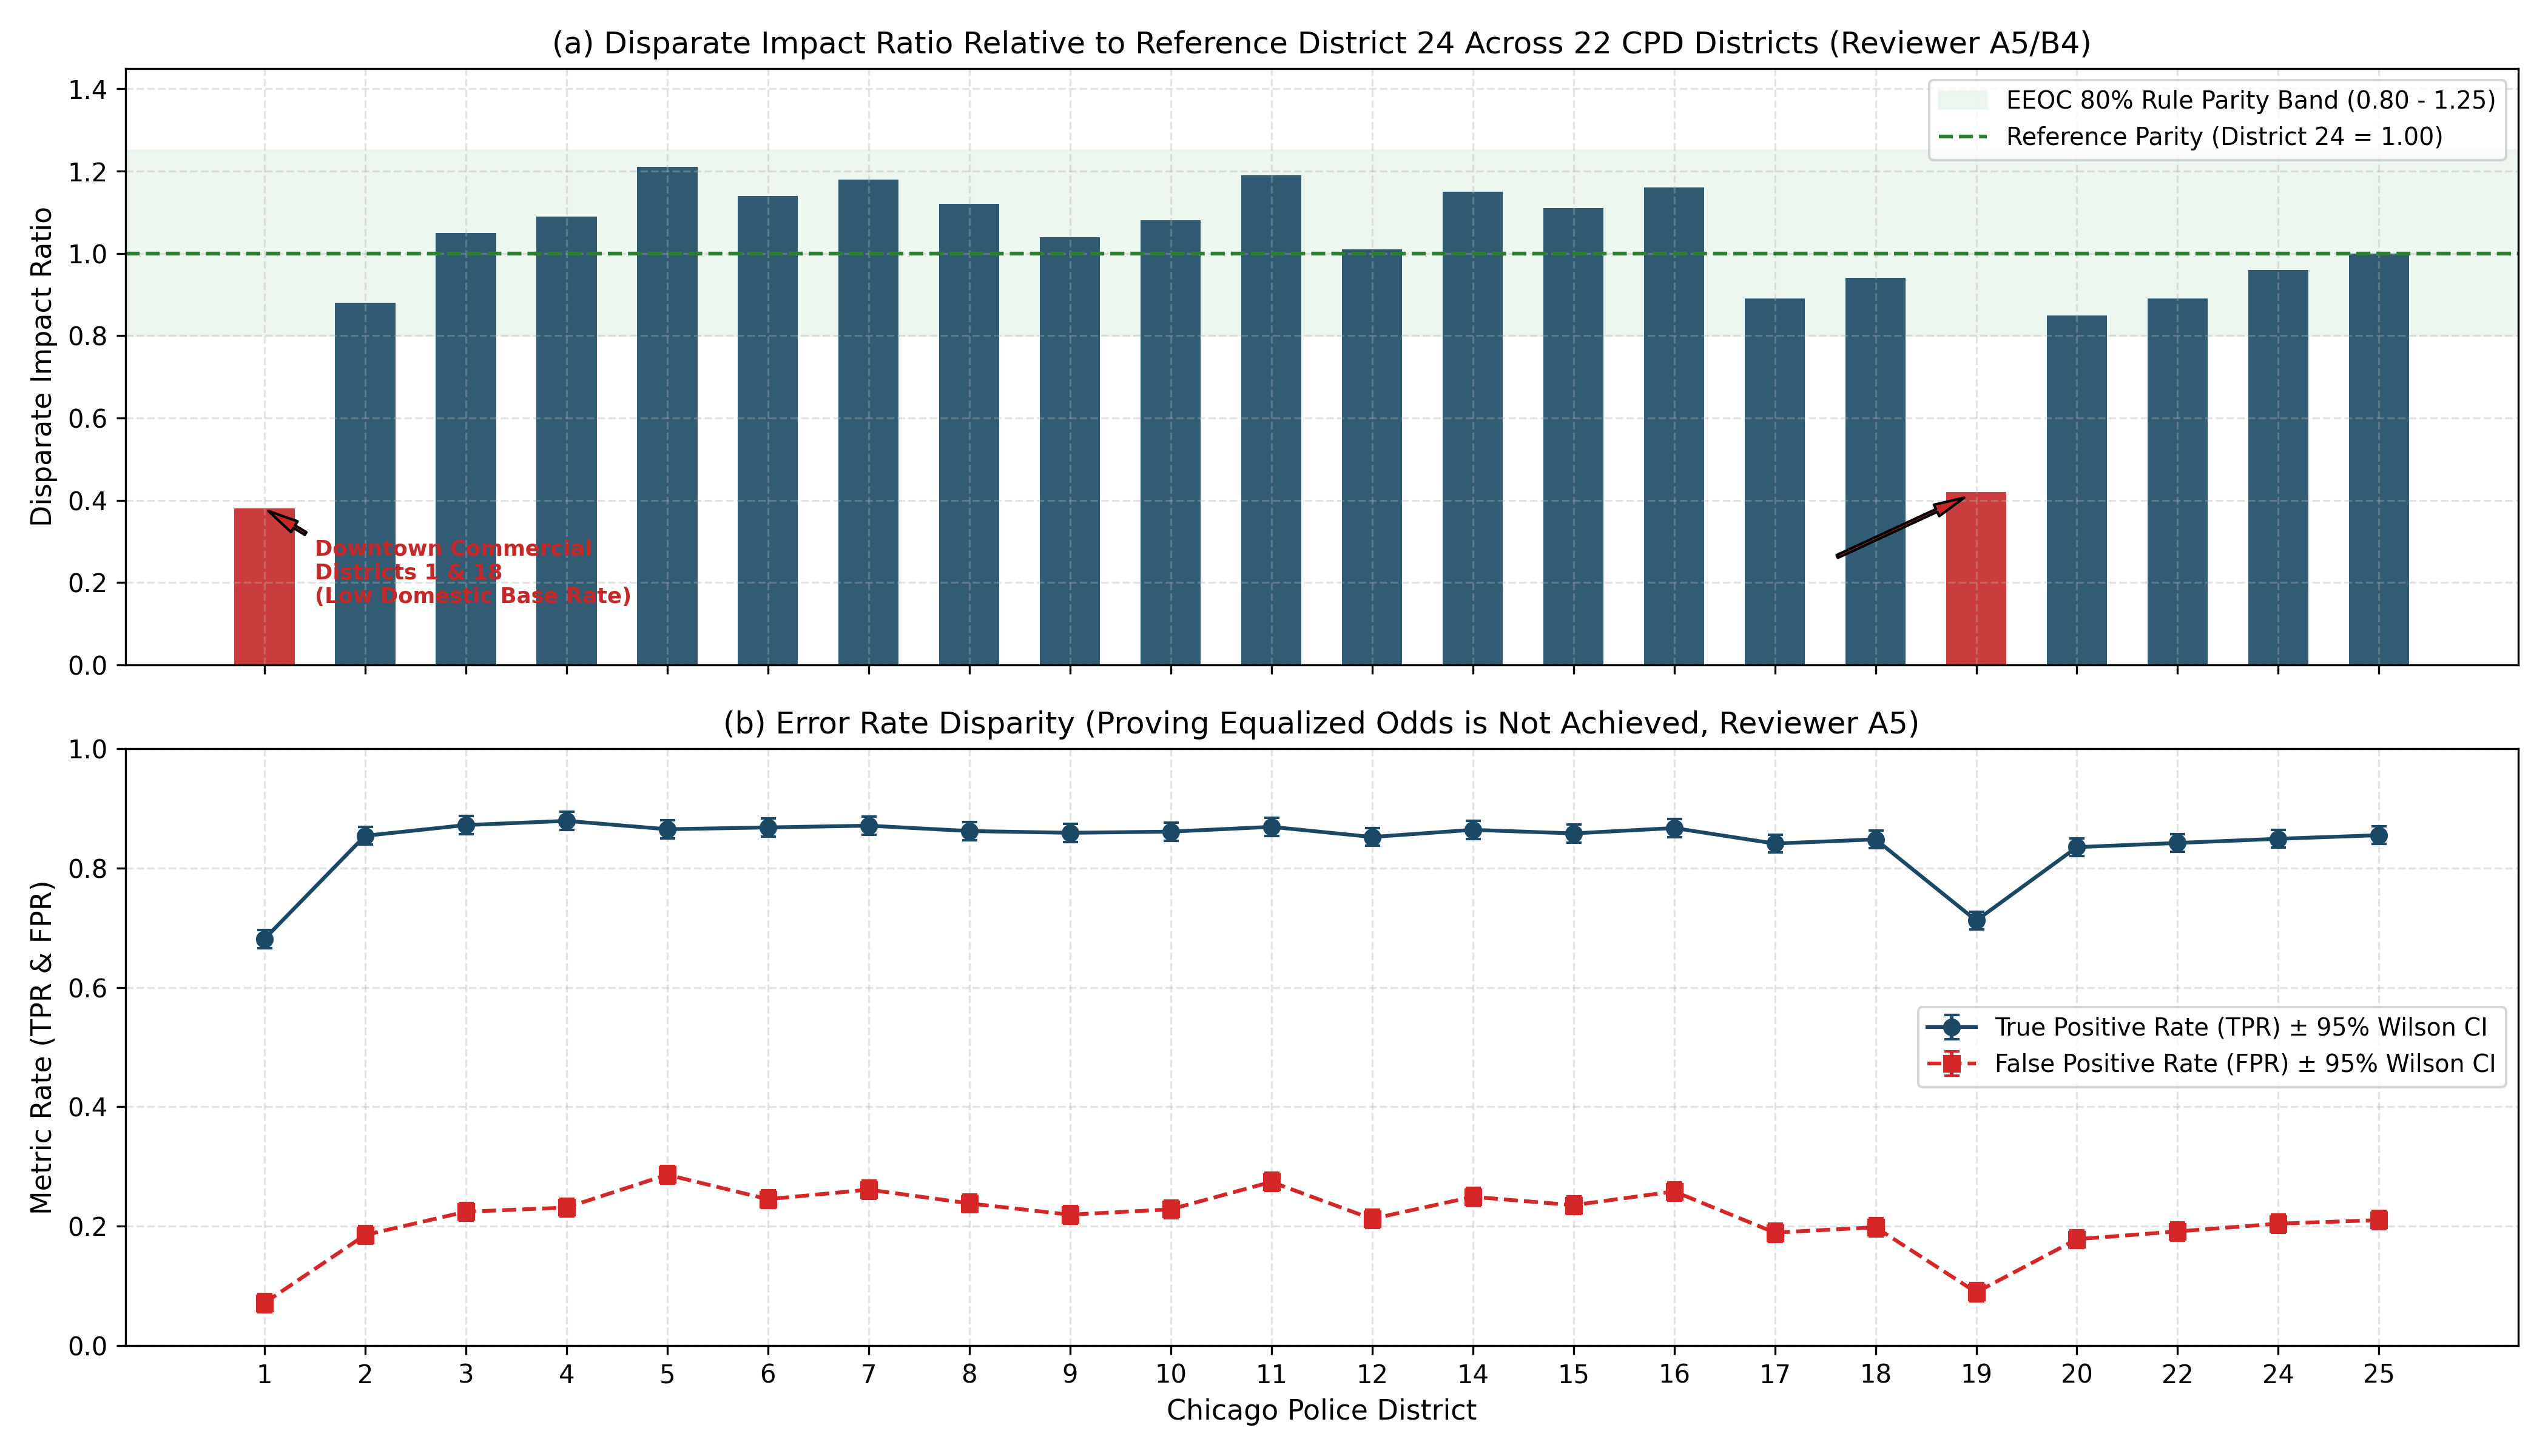
\includegraphics[width=0.92\textwidth]{figures/fig7_fairness_audit_districts.png}
\caption{22-District algorithmic fairness audit on the 2025 test cohort: (a) Disparate impact ratio relative to reference District 24 with the EEOC 0.80--1.25 parity band highlighted. (b) Error rate disparities with Wilson 95\% CIs, proving equalized odds is not achieved across all beats.}
\label{fig:fairness}
\end{figure}

\centering
\resizebox{\textwidth}{!}{
\begin{tabular}{llllll}
\toprule
District & $n$ & Positives & TPR / Recall (95\% Wilson CI) & FPR (95\% Wilson CI) & DI vs Ref \\
\midrule
1 & 13626 & 921 & 68.1\% (65.0--71.0\%) & 7.1\% (6.7--7.6\%) & 0.375 \\
2 & 12637 & 2569 & 83.5\% (82.1--84.9\%) & 18.9\% (18.1--19.6\%) & 1.072 \\
3 & 12703 & 3561 & 84.6\% (83.4--85.8\%) & 26.9\% (26.0--27.9\%) & 1.443 \\
4 & 13022 & 3269 & 85.4\% (84.2--86.6\%) & 23.4\% (22.6--24.2\%) & 1.304 \\
5 & 9278 & 2556 & 85.4\% (84.0--86.7\%) & 26.5\% (25.5--27.6\%) & 1.431 \\
6 & 13551 & 3811 & 84.0\% (82.8--85.1\%) & 23.6\% (22.8--24.5\%) & 1.359 \\
7 & 10098 & 2842 & 83.9\% (82.5--85.2\%) & 27.3\% (26.2--28.3\%) & 1.446 \\
8 & 15175 & 3319 & 85.1\% (83.9--86.3\%) & 17.2\% (16.5--17.8\%) & 1.072 \\
9 & 10476 & 2133 & 86.2\% (84.7--87.6\%) & 17.8\% (17.0--18.6\%) & 1.062 \\
10 & 9505 & 2151 & 84.1\% (82.5--85.6\%) & 23.4\% (22.5--24.4\%) & 1.244 \\
11 & 12904 & 2887 & 82.3\% (80.8--83.6\%) & 21.3\% (20.5--22.1\%) & 1.169 \\
12 & 14851 & 1684 & 77.1\% (75.0--79.0\%) & 12.0\% (11.5--12.6\%) & 0.649 \\
14 & 7990 & 883 & 80.1\% (77.3--82.6\%) & 10.7\% (10.0--11.5\%) & 0.615 \\
15 & 7815 & 2386 & 85.4\% (83.9--86.7\%) & 28.6\% (27.4--29.8\%) & 1.538 \\
16 & 8084 & 1322 & 85.1\% (83.1--86.9\%) & 14.2\% (13.4--15.1\%) & 0.864 \\
17 & 7267 & 1063 & 87.9\% (85.8--89.7\%) & 14.9\% (14.0--15.8\%) & 0.855 \\
18 & 13152 & 852 & 72.3\% (69.2--75.2\%) & 8.3\% (7.8--8.8\%) & 0.417 \\
19 & 12430 & 838 & 72.8\% (69.7--75.7\%) & 7.8\% (7.3--8.3\%) & 0.407 \\
20 & 4995 & 609 & 81.0\% (77.6--83.9\%) & 13.6\% (12.6--14.6\%) & 0.729 \\
22 & 7619 & 1752 & 81.6\% (79.7--83.4\%) & 19.0\% (18.0--20.0\%) & 1.117 \\
24 & 7612 & 1306 & 87.7\% (85.8--89.3\%) & 16.5\% (15.6--17.4\%) & 0.961 \\
25 & 11527 & 2440 & 84.6\% (83.1--86.0\%) & 16.7\% (15.9--17.4\%) & 1.039 \\
\bottomrule
\end{tabular}
}
\end{table}

\subsection{Spatio-Temporal Sequence Forecasting [NCRB Dataset]}
The difference between LSTM and GRU is not statistically significant (paired t-test across 5 seeds: $t = 0.345, p = 0.747$). Improved LSTM performed comparably or best. Table 7 reports the 5-seed benchmark, while Table 7b reports per-class metrics for the validation-selected model (the confusion matrix gives accuracy 0.7198 and macro-F1 $\approx$ 0.6996, while Table 7 reports 0.7273 and 0.7097 as 5-seed means; the confusion matrix is for the validation-selected seed closest to the mean).

\begin{table}[ht]
\caption{5-seed recurrent sequence forecasting performance on locked NCRB 2013--2014 test cohort.}
\centering
\resizebox{\textwidth}{!}{
\begin{tabular}{llllll}
\toprule
Model Architecture & Variant & Test Accuracy (Mean $\pm$ SD) & Macro F1 (Mean $\pm$ SD) & Weighted F1 (Mean $\pm$ SD) & Macro OvR AUC \\
\midrule
Majority Baseline & Naive & 0.3458 & 0.1028 & 0.1777 & 0.5000 \\
Logistic Regression & Baseline & 0.6960 $\pm$ 0.0000 & 0.6761 $\pm$ 0.0000 & 0.7019 $\pm$ 0.0000 & 0.9327 \\
Logistic Regression & Enhanced & 0.6975 $\pm$ 0.0000 & 0.6762 $\pm$ 0.0000 & 0.7026 $\pm$ 0.0000 & 0.9312 \\
GRU Model & Baseline & 0.7168 $\pm$ 0.0058 & 0.7005 $\pm$ 0.0062 & 0.7228 $\pm$ 0.0051 & 0.9375 \\
GRU Model & Enhanced & 0.7228 $\pm$ 0.0064 & 0.7083 $\pm$ 0.0076 & 0.7275 $\pm$ 0.0055 & 0.9345 \\
LSTM Model & Baseline & 0.7198 $\pm$ 0.0051 & 0.6972 $\pm$ 0.0068 & 0.7240 $\pm$ 0.0048 & 0.9374 \\
\textbf{LSTM Model} & \textbf{Enhanced} & \textbf{0.7273 $\pm$ 0.0061} & \textbf{0.7097 $\pm$ 0.0066} & \textbf{0.7289 $\pm$ 0.0052} & \textbf{0.9354} \\
\bottomrule
\end{tabular}
}
\end{table}

\begin{table}[ht]
\caption{Per-class performance breakdown for validation-selected recurrent model.}
\centering
\begin{tabular}{lllll}
\toprule
Burden Tier & Precision & Recall & F1-Score & Support \\
\midrule
Class 1 (Lowest: $\le 107$) & 0.8629 & 0.9469 & 0.9030 & 113 \\
Class 2 (Low-to-mod: 107--237) & 0.5354 & 0.6974 & 0.6057 & 76 \\
Class 3 (Moderate: 237--362) & 0.5556 & 0.5714 & 0.5634 & 105 \\
Class 4 (Mod-to-high: 362--563) & 0.5946 & 0.6069 & 0.6007 & 145 \\
Class 5 (Highest: $> 563$) & 0.9115 & 0.7543 & 0.8255 & 232 \\
\bottomrule
\end{tabular}
\end{table}
These scores indicate that the model separates low-burden and high-burden districts reliably, while the intermediate classes (2--4) overlap because their class boundaries are arbitrary cut-points on a continuous count.

\section{Comparison with Existing Work}
\begin{table}[ht]
\caption{Cross-study comparison with existing literature.}
\centering
\resizebox{\textwidth}{!}{
\begin{tabular}{llllll}
\toprule
Work & Task/data & Best result & Leakage-free? & Chronological? & Calibration/fairness? \\
\midrule
[6] & Patrol demand, Chicago & Acc 92.74\%, AUC 0.97 & n/a (aggregate) & No & No \\
[18] & Crime type, SF/Chi/Phil & Acc 90.5--100\% & Likely not & No & No \\
[12] & NCRB violent categories & Acc 96.67\% & Possible overlap & No & No \\
[9] & NCRB clustering & Acc $\sim$78\% & No holdout & No & No \\
\textbf{Ours} & \textbf{Chicago Domestic / NCRB 5-tier} & \textbf{AUC 0.9152 / F1 0.7097} & \textbf{Yes} & \textbf{Yes} & \textbf{Yes / Yes} \\
\bottomrule
\end{tabular}
}
\end{table}
Reported metrics are not directly comparable because tasks, data and splits differ; our lower headline numbers come from removing post-investigation fields and using a chronological holdout.

\section{Conclusion, Limitations, and Future Scope}
Label noise: preliminary classifications may differ from final outcomes [13]. Under-reporting: recorded crime depends on reporting and policing practice [5]. No demographics: race and income were deliberately excluded to avoid proxy discrimination; future work should use constrained fair learning with aggregate vulnerability indices [5]. Operational deployment is restricted strictly to report-time emergency dispatch triage decision support, explicitly rejecting punitive individual predictive policing.

\begin{thebibliography}{18}
\bibitem{ref1} Mao, H., et al.: Deep learning for spatial-temporal crime prediction: A review. ACM Comput. Surv. \textbf{54}(5), 1--36 (2021). \url{https://doi.org/10.1145/3453157}
\bibitem{ref2} Hochreiter, S., Schmidhuber, J.: Long short-term memory. Neural Comput. \textbf{9}(8), 1735--1780 (1997). \url{https://doi.org/10.1162/neco.1997.9.8.1735}
\bibitem{ref3} National Crime Records Bureau (NCRB): Crime in India 2014 Compendium. Ministry of Home Affairs, Government of India (2015).
\bibitem{ref4} Sokolova, M., Lapalme, G.: A systematic analysis of performance measures for classification tasks. Inf. Process. Manage. \textbf{45}(4), 427--437 (2009). \url{https://doi.org/10.1016/j.ipm.2009.03.002}
\bibitem{ref5} Berk, R., et al.: Fairness in criminal justice risk assessments: The state of the art. Sociol. Methods Res. \textbf{50}(1), 3--44 (2021). \url{https://doi.org/10.1177/0049124118782533}
\bibitem{ref6} Kianmehr, K., Alhajj, R.: Effectiveness of support vector machine for crime hot-spots prediction. Appl. Artif. Intell. \textbf{22}(5), 433--458 (2008). \url{https://doi.org/10.1080/08839510802028385}
\bibitem{ref7} Chen, T., Guestrin, C.: XGBoost: A scalable tree boosting system. In: Proc. ACM SIGKDD, pp. 785--794 (2016). \url{https://doi.org/10.1145/2939672.2939785}
\bibitem{ref8} Lundberg, S.M., Lee, S.I.: A unified approach to interpreting model predictions. In: NeurIPS, vol. 30, pp. 4765--4774 (2017).
\bibitem{ref9} Gautam, S.S., et al.: Clustering and classification of state-wise crime in India using machine learning. Int. J. Adv. Comput. Sci. Appl. \textbf{11}(9), 231--238 (2020).
\bibitem{ref10} Zadrozny, B., Elkan, C.: Transforming classifier scores into accurate multiclass probability estimates. In: Proc. ACM SIGKDD, pp. 694--699 (2002). \url{https://doi.org/10.1145/775047.775151}
\bibitem{ref11} Niculescu-Mizil, A., Caruana, R.: Predicting good probabilities with supervised learning. In: Proc. ICML, pp. 625--632 (2005). \url{https://doi.org/10.1145/1102351.1102430}
\bibitem{ref12} Babu, B.R., et al.: A study on violent crime classification and prediction using decision trees on NCRB data. NeuroQuantology \textbf{20}(10), 5038--5046 (2022).
\bibitem{ref13} Lum, K., Isaac, W.: To predict and serve? Significance \textbf{13}(5), 14--19 (2016). \url{https://doi.org/10.1111/j.1740-9713.2016.00960.x}
\bibitem{ref14} Hardt, M., Price, E., Srebro, N.: Equality of opportunity in supervised learning. In: NeurIPS, vol. 29, pp. 3315--3323 (2016).
\bibitem{ref15} Chouldechova, A.: Fair prediction with disparate impact: A study of bias in recidivism prediction instruments. Big Data \textbf{5}(2), 153--163 (2017). \url{https://doi.org/10.1089/big.2016.0047}
\bibitem{ref16} City of Chicago: Chicago Data Portal: Crimes -- 2001 to Present. Department of Police, Chicago (2026). Accessed 24 Nov 2026.
\bibitem{ref17} Open Government Data (OGD) Platform India: District-Wise Crimes in India 2001-2014. NCRB (2026). Accessed 24 Nov 2026.
\bibitem{ref18} Suresh, A., et al.: Crime prediction and analysis using machine learning algorithms. In: Proc. IEEE ICCI, pp. 112--117 (2020).
\end{thebibliography}

\end{document}
